\documentclass{article}


\usepackage[top=2in, bottom=1.5in, left=1in, right=1in]{geometry}
\usepackage{amssymb,amsmath}

\usepackage{algorithm}
\usepackage{algpseudocode}

\usepackage{graphicx}


\usepackage{natbib}

\makeatletter
\newcommand{\xRightarrow}[2][]{\ext@arrow 0359\Rightarrowfill@{#1}{#2}}
\makeatother

\newcommand{\derives}{\xRightarrow{*}}


\author{Eyal Dechter}

\begin{document}
The Inside-Outside algorithm is a popular algorithm for computing the
MAP marginals of PCFG rules given a sentence or collection of
sentences. The algorithm's computational complexity is $O(n^3 K)$
where $n$ is the length of the sentence and $K$ is the the number of
rules in the PCFG. The cubic algorithm makes inference tractable for
relatively long sentences -- containing perhaps a few dozen terminals
-- but makes it impossible for this algorithm to be used in an online
fashion, or to be used on grammars that span multiple levels of
linguistic abstration (for example, imagine trying to learn
morphological and syntactic grammar at the same time with the
Inside-Outside algorithm). 

Our goal here is to develop an algorithm that approximates the MAP
marginals of a PCFG given data but that can run much faster; further,
we would like to be able to put bounds on the approximation. The core
intuition is that if we know that the probability of some symbol
dominating a span cannot be more than some very small amount, we
shouldn't have to calculate that amount accurately; instead, we should
be able to substitute this small upperbound in our calculations,
absolving us of exploring parts of the space of parses that are very
unlikely to be relevant.

In what follows we will assume that we have a PCFG $G$ in Chomsky
normal form with start symbol $S$, non-terminals $\mathcal{A}$,
terminals $\mathcal{T}$, and rules $\mathcal{R}$, where we associate
with each rule $r \in \mathcal{R}$ a potential $\psi(r)$. We also
assume that we are given a sentence $x = x_1, \dots, x_N$.

For every triple $(A, i, j)$ where $A$ is a nonterminal and $1 \leq i
\leq j \leq N$, the Inside-Outside algorithm computes an alpha and
beta value. The alpha and beta values are defined according to the
following recurrence:

\begin{align}
\alpha(A, i, i) &= \psi(A \rightarrow x_i)\\
\alpha(A, i, j) &= \sum_{k=i}^{j-1} \sum_{A \rightarrow B C \in \mathcal{R}}
  \psi(A \rightarrow B C ) \alpha(B, i, k) \alpha(C, k+1, j)\\
\beta(A, 1, N) &= 1 \\
\beta(A, i, j) &= \sum_{k=1}^{i-1} \sum_{B \rightarrow C A \in \mathcal{R}}
  \beta(B, k, j) \psi(B \rightarrow C A) \alpha(C, k, i-1)\\ 
  &+  \sum_{k=j+1}^{N} \sum_{B \rightarrow A C \in \mathcal{R} : A \neq C}
  \beta(B, i, k) \psi(B \rightarrow A C) \alpha(C, j+1, k) 
\end{align}

Suppose we have an approximate $\alpha'$ of $\alpha$ with the
property that for some small $\epsilon > 0$ and for all $A, i, j$: 

\begin{align}
\alpha'(A, i, i) &= \alpha(A, i, i)\\ 
\alpha(A, i, j) &\leq \alpha'(A, i, j) \leq (1+\epsilon)  \sum_{k=i}^{j-1} \sum_{A \rightarrow B C \in \mathcal{R}} 
  \psi(A \rightarrow B C ) \alpha'(B, i, k) \alpha'(C, k+1, j).\\
\end{align}

By how much can $\alpha'$ over estimate $\alpha$? Let $E(A, i,
j)=\frac{\alpha'(A, i, j)}{\alpha(A, i, j)}$ be the measure of this
over-estimate. We have that 

\begin{align}
E_{\alpha}(A, i, i) &= 1\\
E_{\alpha}(A, i,j) &= \frac{\alpha'(A, i, j)}{\alpha(A, i, j)}\\
          &\leq (1+\epsilon) \frac{ \sum_{k=i}^{j-1} \sum_{A \rightarrow B C \in \mathcal{R}} 
  \psi(A \rightarrow B C ) \alpha'(B, i, k) \alpha'(C, k+1, j)}
           {\sum_{k=i}^{j-1} \sum_{A \rightarrow B C \in \mathcal{R}}
  \psi(A \rightarrow B C ) \alpha(B, i, k) \alpha(C, k+1, j)}\\
          &=  (1+\epsilon) \frac{ \sum_{k=i}^{j-1} \sum_{A \rightarrow B C \in \mathcal{R}} 
  \psi(A \rightarrow B C ) E_{\alpha}(B, i, k) \alpha(B, i, k) E_{\alpha}(C, k+1, j) \alpha(C, k+1, j)}
           {\sum_{k=i}^{j-1} \sum_{A \rightarrow B C \in \mathcal{R}}
  \psi(A \rightarrow B C ) \alpha(B, i, k) \alpha(C, k+1, j)}\\
         &= (1+\epsilon) \max_{k\in \{i, \dots, j-1\}, A \rightarrow B C \in \mathcal{R} }
            E_{\alpha}(B, i, k) E_{\alpha}(C, k+1, j).
\end{align}

Let $\hat{E}_{\alpha}(d) = \max_{A\in\mathcal{A}, i \in \{1, \dots, N-d \}}
E_{\alpha}(A, i, i+d)$ be the maximum upper bound above over all spans of
length $d$. Then we have that

\begin{align}
\hat{E}_{\alpha}(1) &= 1\\
\hat{E}_{\alpha}(d) &= (1+\epsilon) \max_{s \in \{1, \dots, d-1\}} \hat{E}_{\alpha}(s) \hat{E}_{\alpha}(d-s).\\
\end{align}

Solving this recurrence, gives $\hat{E}_{\alpha}(d) = (1 + \epsilon)^{d-1}$. To
re-iterate, what this means is that if we have such an $\alpha'$ then
for all $A, i, j$, $\alpha'(A, i, j) \leq (1 + \epsilon)^{j - i}
\alpha(A, i, j)$.

We can now develop an analog $\beta'$ of $\beta$ which has the same
dependency on $\alpha'$ that $\beta$ has on $\alpha$. Let
$\hat{E}_{\beta}(d)$ be an upper bound on $\frac{\beta'(A, i,
  i+d)}{\beta(A, i, i+d)}$ for all $A$ and $i$. Then a similar
analysis as above shows that one such $\hat{E}_\beta$ is

\begin{align}
\hat{E}_{\beta}(N) &= 1\\
\hat{E}_{\beta}(N-k) &= (1+\epsilon)^{N-k-1} \max_{s \in \{N-k+1, \dots, N\}} \hat{E}_{\beta}(s).
\end{align}

Solving this recurrence yields $\hat{E}_{\beta}(d) = (1+\epsilon)^{\frac{(N-d)(N+d-1)}{2}}$.

In the Inside-Outside algorithm, the merit $\mu(A, i, j) = \alpha(A,
i, j) \beta(A, i, j)$ is the unnormalized probability that nonterminal
$A$ yields span $(i, j)$. Define $\mu'(A, i, j) = \alpha'(A, i, j)
\beta(A, i, j)$. By the results above, we have that the ratio of the
actual merit to our approximation is upper bounded by
$(1+\epsilon)^{\frac{(N+d-2)(N-d+1)}{2}}$, where, as before, $d$ is
the length of the span $(i, j)$.


\section{Approximate Inside}
Here we describe the algorithm ApproxInside which computes the
$\alpha'$ values.


\begin{algorithm}
\caption{The Approximate Inside Algorithm \label{alg:approxInside}}
\begin{algorithmic}[1]
\Procedure {ApproxInside}{$s$, $G=(S, bRules, uRules)$, $U$, $\epsilon$}
  \State \Comment $s$ sentences of length $n$
  \State \Comment $G$ grammar 
  \State \Comment $S$ start symbol
  \State \Comment $U$ upper bound, function from $(A, i, j) \mapsto \mathbf{R}$
  \State $\alpha \leftarrow \Call{InitAlpha}{G, 1, n}$ \Comment Initialize table of $\alpha$ 
  \State \Return \Call{$GO_{OR}$}{$S$, $1$, $n$}
\EndProcedure
\end{algorithmic}
\end{algorithm}

\begin{algorithm}
\caption{The Approximate Inside Algorithm (cont)}
\begin{algorithmic}[2]
\Procedure {$GO_{OR}$}{$A$, $i$, $j$}
  \State \Comment $A$ nonterminal symbol
  \State $children \leftarrow \Call{GetChildren}{A, i, k}$
  \State $lb \leftarrow 0 $ \Comment Initialize lower bound on OR node to 0
  \For{$node \in children$}{}{}
    \If{$node$ is unary of form $A \rightarrow t, i, i$ and $t = s_i$}
      \State $v \leftarrow \psi(A \rightarrow t)$
    \ElsIf{$node$ is binary}
      \State $v \leftarrow $\;\Call{$GO_{AND}$}{$node$, $lb$}
    \EndIf
    \State $lb \leftarrow lb + v$ \Comment Update lower bound
  \EndFor
  \State $\alpha[A, i, j] \leftarrow lb$ \Comment Insert $\alpha$ value into table.
\EndProcedure
\Statex
\Procedure {$GO_{AND}$}{$A \rightarrow B\, C$, $i$, $k$,$j$, $lb$}
  \State $w \leftarrow \psi(A \rightarrow B\, C)$ 
  \State $v_{\ell} \leftarrow \alpha[B, i, k]$ 
  \State $v_{r} \leftarrow \alpha[C, k+1, j]$
  \State $u_{\ell} \leftarrow U[B, i, k]$ 
  \State $u_{r} \leftarrow U[C, k+1, j]$
  \If{neither $v_{\ell}$ nor $v_r$ is $NIL$} \Comment If both values are already computed, just use them
    \State \Return $w * v_{\ell} * v_r$
  \ElsIf{ $v_r \neq NIL$}  \Comment If the right value is already computed, compute left value
    \If {$u_\ell \leq \frac{\epsilon * lb}{w * v_r}$}
      \State $v_\ell \leftarrow u_\ell$
    \Else
      \State $v_\ell \leftarrow $\;\Call{$GO_{OR}$}{$B$, $i$, $k$}
    \EndIf
  \ElsIf{ $v_\ell \neq NIL$}  \Comment If the left value is already computed, compute right value
    \If {$u_r \leq \frac{\epsilon * lb}{w * v_\ell}$}
      \State $v_r \leftarrow u_r$
    \Else
      \State $v_r \leftarrow $\;\Call{$GO_{OR}$}{$C$, $k+1$, $j$}
    \EndIf
  \Else \Comment If neither values yet computed, compute both
    \If {$u_\ell u_r \leq \frac{\epsilon * lb}{w}$}
      \State $v_r \leftarrow u_r$
      \State $v_\ell \leftarrow u_\ell$
    \Else
      \State $v_\ell \leftarrow $\;\Call{$GO_{OR}$}{$B$, $i$, $k$}
      \State $v_r \leftarrow $\;\Call{$GO_{OR}$}{$C$, $k+1$, $j$}
    \EndIf
  \EndIf
  \State \Return $w * v_{\ell} * v_r$
\EndProcedure
\end{algorithmic}
\end{algorithm}


\begin{algorithm}
\caption{The Approximate Outside Algorithm.\label{alg:approxOutside}}
\begin{algorithmic}[2]
\Procedure {$ApproxOutside$}{$s$, $G$, $S$}
  \State $n \leftarrow length(s)$
  \State $\beta[S, 1, n] \leftarrow 1$ \Comment initialize $\beta$ recursion, unless $n==1$ in which case we are done
  \For {$\ell \gets 1, \dots, n-1$}
    \For {$i \gets \ell$}
      \State $j \leftarrow i + \ell$
    \EndFor
  \EndFor

  \State $open \leftarrow [(S, 1, n)]$ \Comment initialize list that will hold nodes to be processed
  \While {$open \neq NIL$}
  \State $children \leftarrow []$ \Comment initialize list that holds next level of nodes to be processed
   \For {$(A, i, j) \in open$ \Comment $i \neq j$}
    \For {$A \leftarrow B\, C \in rules(G)$} \Comment iterate over binary rules headed by $A$
      \For {$k \leftarrow i, \dots, j - 1$}
        \If {$\alpha[B, i, k] \neq 0$}
          \State if $\beta[C, k+1, j] = NIL$, set to $0$
          \State $\beta[C, k+1, j] \leftarrow \beta[C, k+1, j] + \psi(A \rightarrow B C) \alpha[B, i, k] \beta[A, i, j]$
          \State add $(C, k+1, j)$ to $children$
        \EndIf 

        \If {$\alpha[C, k+1, j] \neq 0$}
          \State if $\beta[B, i, k] = NIL$, set to $0$
          \State $\beta[B, i, k] \leftarrow \beta[B, i, k] + \psi(A \rightarrow B C) \alpha[C, k+1, j] \beta[A, i, j]$
          \State add $(B, i, k)$ to $children$
        \EndIf 
      \EndFor 
   \EndFor
   \EndFor
   \State $open \leftarrow children$
  \EndWhile    
\EndProcedure
\end{algorithmic}
\end{algorithm}


\noindent \textbf{Claim: Algorithm~\ref{alg:approxInside} correctly computes the $\beta'$ values.}
\noindent TODO

\noindent \textbf{Claim: Algorithm~\ref{alg:approxOutside} correctly computes the $\beta'$ values.}
\noindent TODO

The algorithm presented provides two degrees of freedom to the user: the first is a choice of upperbound function $U$, and the second is a way to order the children of a node. The tighter the upperbound, the better an approximation we get. The better the ordering of the children, the less often we need to explore derivations of low relative weight. 


\section{Ordering heuristics}
How we order the children of a node is critical to the speed-up this
aproximate algorithm gets. After all, if there is a child whose
derivation dominates all others and we accidentally put it last, then
we will not be able to short-circuit at all; if, instead, we put it
first, then we will likely only have to explore that child.

One can image various choices of ordering functions, with perhaps the
simplest being to pick the rules in order of decreasing weight. This,
however, only gives us an ordering on the rules, not on where we
should split the span of the child. One reasonable suggestion,
especially for right branching structures like English parse trees, is
to start with the smallest left child spans first and increase from
there.

These heuristics, however, are very weak, and do not take into
consideration the content span at all. In the following we propose a
simple heuristic with child ordering that takes into account the
bottom-up probability of the content but whose complexity is constant
in the size of the span. The basic intutiion behind this heuristic is
that if one wants to evaluate the probability that, e.g., a noun
phrase will yield that fragmant ``saw the boy with,'' one can gain a
lot of information by calculating the probability that the phrase will
start and end with ``saw'' and ``with,'' respectively. 

Some notation: let's denote by $\gamma(A, x)$ the probability that a
nonterminal $A$ derives any string with prefix $x$. Likewise, let's
denote by $\theta(A, x)$ the proabability that a nonterminal $A$
derives any string with suffix $x$. We will write this using the
following notation:

\begin{align}
  \gamma(A, x) &\triangleq p(A \xRightarrow{*} x\dots) \label{eq:gammaDef}\\
  \theta(A, x) &\triangleq p(A \xRightarrow{*} \dots x)  \label{eq:thetaDef}
\end{align}

$\gamma(A, x)$ is just the prefix probability defined for a single
lexical item. This can be defined as:
\begin{align}
  p(A \derives x\dots) &= \sum_{A \rightarrow BC} p(B \derives x \dots) p(A \rightarrow B C) 
    + p(A \rightarrow x)\\
  p(A \derives \dots x) &= \sum_{A \rightarrow CB} p(B \derives \dots x) p(A \rightarrow C B) 
    + p(A \rightarrow x)
\end{align}

If we define the matrices $\Gamma$ and $\Theta$ where $\Gamma_{A, B} = \gamma(A, B)$
and $\Theta_{A, B} = \theta(A, B)$. then we can rewrite these recursions 

\begin{align}
  \Gamma &= \Phi^\ell \Gamma + \Psi \\
  \Theta &= \Phi^r \Gamma  + \Psi \\
  \text{where }\Phi^\ell_{A, B} &\triangleq \sum_{A \rightarrow B C} p(A \rightarrow B C)\\
               \Phi^r_{A, B} &\triangleq \sum_{A \rightarrow C B} p(A \rightarrow C B)\\
               \Psi_{A, x} &\triangleq p(A \rightarrow x).
\end{align}

This means that we can calculate $\Gamma$ and $\Phi$ by solving the linear systems 

\begin{align}
  (1-\Phi_\ell) \Gamma &= \Psi\\
  (1-\Phi_r) \Theta &= \Psi.\\
\end{align}

The complexity of these calculations is $K^3$, where $K$ is the number
of symbols in the grammar. 

From $\Gamma$ and $\Theta$ we can compute the boundary probability: 
\begin{align}
  p(A \derives x \dots y) &= p(A \rightarrow x) \mathbf{1}(x = y) 
     + \sum_{A \rightarrow B C} p(A \rightarrow B C) p(B \derives x \dots) p(C \derives \dots y)\\
  p(A \derives x \dots y) &= p(A \rightarrow x) \mathbf{1}(x = y) 
     + \sum_{A \rightarrow B C} p(A \rightarrow B C) \Gamma_{B, x} \Theta_{y, C}
\end{align}

Here, as is often the case in computations that make use of heuristic
scores, it may be advantageous to precompute all the heuristic values
so that lookup is $O(1)$. 

\subsection{A serious problem with boundary probabilities}
Unfortunately, there is are serious problems with using boundary
probabilities. First, the dependency between the first and last word
of a constituent decreases rapidly with the length of the
constitutent. Second, since calculating the boundary probability
involves taking the expectation over yields of all lengths, the value
assigned does not take into accoutn the length of the constitutent,
and produces values that upper bound the insid probability of a
consituent even for two word constitutent. But even an unlikely pair
of adjacent words is going to have a higher probability than a typical
long sentence. Therefore, we need to come up with a scoring function
that takes into account the length of the constitutent.

\section{Using constituent length to upper bound inside probabilities}
The probability that symbol $A$ yields any constitutent of length $n$
is greater than or equal to the probability that symbol $A$ yields any
specific string of words of that length. 

Let $\lambda(A, n) \triangleq p(A \text{ yields a string of lengths }
n)$. This probability can be calculated recursively: 
\begin{align}
\lambda(A, n=1) =& \sum_{A \leftarrow t} \psi(A \leftarrow t)\\ 
\lambda(A, n>1) =& \sum_{A \leftarrow B \,C} \sum_{k=1}^{n-1} \psi(A \leftarrow B\, C) 
  \lambda(B, k) \lambda(C, k=1)\\ 
\end{align}

This recursive definition leads directly to an $O(Kn^2)$ algorithm for
$\lambda$. 

\begin{figure}
\begin{minipage}[t]{\textwidth}
  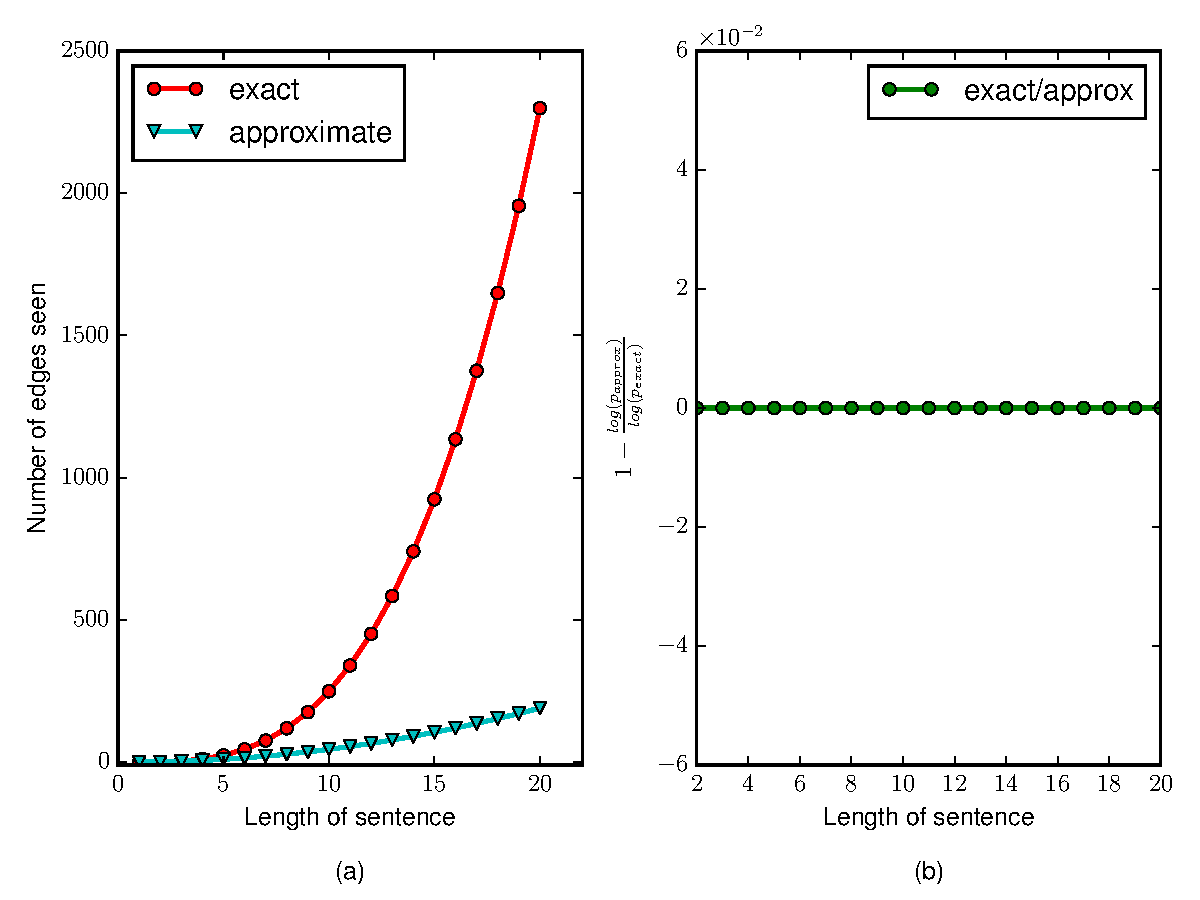
\includegraphics[width=\linewidth]{figures/toy_grammar_approx_vs_exact.pdf}
\end{minipage}
\begin{minipage}[t]{4cm}
  \begin{align*}
    S \rightarrow& \,L\, S :: 0.1 \, | \,a :: 0.9\\
    L \rightarrow& \,L\, S :: 0.0001\, | \, a :: 0.999\\
  \end{align*}
  \centering (a)\par
\end{minipage}

\begin{minipage}[t]{\textwidth}
  \caption{A comparison of the approximate and exact ``Inside''
    algorithms on the toy grammar (c). (a) The number of edges seen by
    the algorithm. The exact Inside algorithm has a predictable $n^3$
    behavior because it looks once at every edge $(A, i, k, j)$. The
    approximate algorithm ignores edges that are gauranteed to be
    insignificant, so that the number of inspected edges is
    dramatically reduced. (b) The amount by which the approximate
    Inside algorithm over estimates the loglikelihood of the
    sentence. }
\end{minipage}
\end{figure}

\section{Appendix}
\subsection{Existence of $\Gamma$ and $\Theta$}
\textbf{Claim: } The matrices $\Gamma$ and $\Theta$ defined by
Equations~\ref{eq:gammaDef}-\ref{eq:thetaDef} exist.  \textbf{Proof: }
The $\Gamma$ and $\Theta$ matrices will not exist only if
$1-\Phi^\ell$ and $1-\Phi^r$ are singular. To show that they are not
singular we will show that there is no non-zero linear combination of
their columns that sums to zero. The proofs are nearly identical for
$1-\Phi^\ell$ and $1-Phi^r$. 

Suppose, by contradiction, that their is some linear combination $a_1,
..., a_K$ such that $(1-\Phi^\ell) a = 0$. This implies that each $a_i
= \sum_{j} \Phi^\ell_{i, j} a_j$. Recall that the element of
$\Phi^\ell_{A, B} = \sum_{A \rightarrow B C} p(A \rightarrow B C)$,
where $A$ and $B$ are nonterminals. For the PCFG defined by these
probabilities to be valid, $\Phi^\ell_{A,B}$ must be less than
one. Otherwise, there would be a nonzero probability of an infinite
string. Taking the absolute values of both sides of the equation
above, we see that $|{a_i}| \leq \sum_{j} \Phi^\ell_{i, j} |
a_j|$. But if this is true, then  TODO

\bibliographystyle{bibliographystyle}
\bibliography{main}








\end{document}
